\chapter{Árboles Generales}
Un árbol general es aquel que cuyos nodos son de cualquier grado, es decir, pueden tener un número cualquiera de hijos, a diferencia de los árboles binarios que son de grado (0,1 ó 2).

Otra gran diferencia de los árboles generales frente a los árboles binarios es que en nuestro TAD no hablamos de hijos derechos, si no de hermanos derechos de un nodo, por tanto, tendremos nodos que son padre, hijo izquierdo y hermanos derechos, véase en\\ (\textit{Figura 3.1: Estructura de un árbol general}).

\begin{figure}[h]
  \begin{center}
    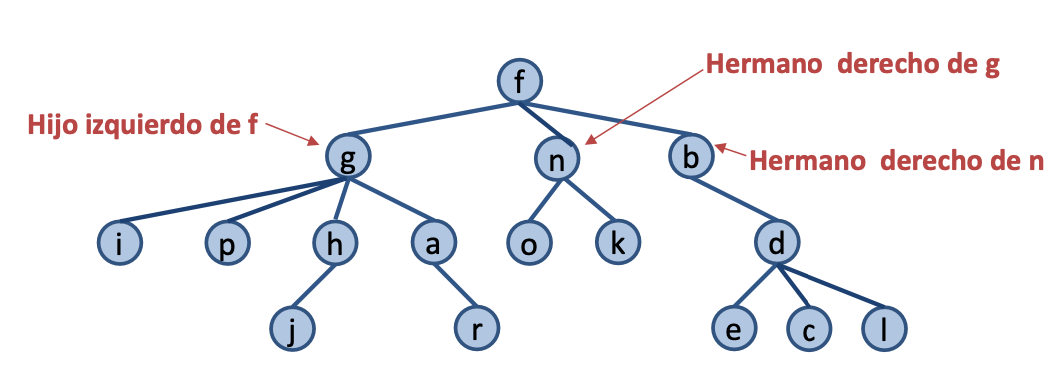
\includegraphics[width=\textwidth]{assets/Agen1.png}
  \end{center}
  \caption[short]{Estructura de un árbol general}
\end{figure}

La creación de un árbol general es igual que en los árboles binarios, partimos de un árbol general vacío e insertamos la raíz y a partir de ahí construimos el árbol insertando hijos izquierdos y hermanos derechos de esos nodos.

Al igual que en el caso de los árboles binarios vamos a ver cuales son y que hacen las operaciones mediante la \textbf{especificación del TAD árbol general}.
\section{Especificación del TAD árbol general}
Sea la especificación de las operaciones del TAD árbol general (Agen):

\subsection*{Constructor del árbol general}
\underbar{\textit{Postcondición:}} Crea y devuelve un árbol general vacío.\\
\verb|  Agen();|

\subsection*{Inserción de nodos}
\begin{itemize}
  \item \underbar{\large\textbf{Inserción del nodo raíz}}:\\
  \underbar{\textit{Precondición:}} Árbol vacío.\\
  \underbar{\textit{Postcondición:}} Inserta el nodo raíz cuyo contenido es `e'.\\
  \verb|  void insertarRaiz(const T& e);|

  \item \underbar{\large\textbf{Inserción de los nodos hijos}}:\\
  \underbar{\textit{Precondición:}} n es un nodo que existe en el árbol.\\
  \underbar{\textit{Postcondición:}} Inserta el elemento `e' como hijo izquierdo de n, si ya tiene un hijo izquierdo el nodo n, este lo inserta y el anterior pasa a ser hermano derecho del nuevo.\\
  \verb|  void insertarHijoIzqdo(nodo n, const T& e);|

  \item \underbar{\large\textbf{Inserción de los nodos hermanos}}:\\
  \underbar{\textit{Precondición:}} n es un nodo que existe en el árbol y no es raíz.\\
  \underbar{\textit{Postcondición:}} Inserta el elemento `e' como hermano derecho del nodo n.\\
  \verb|  void insertarHermDrcho(nodo n,const T& e);|
\end{itemize}
\subsection*{Eliminación de nodos}
Al igual que en los árboles binarios, tenemos que comprobar que el nodo que vamos a eliminar sea una hoja, ya sea un hijo izquierdo o un hermano derecho de un nodo cualquiera.
\begin{itemize}
  \item \underbar{\large\textbf{Eliminación del nodo raíz}}:\\
  \underbar{\textit{Precondición:}} Árbol no vacío y nodo raíz es una hoja.\\
  \underbar{\textit{Postcondición:}} Elimina el nodo raíz y deja el árbol vacío.\\
  \verb|  void eliminarRaiz();|
  \item \underbar{\large\textbf{Eliminación de nodo hijo izquierdo}}:\\
  \underbar{\textit{Precondición:}} n es un nodo del árbol, tiene hijo izquierdo y este es Hoja.\\
  \underbar{\textit{Postcondición:}} Elimina el hijo izquierdo del nodo n y su hermano derecho pasa a ser el nuevo hijo izquierdo.\\
  \verb|  void eliminarHijoIzqdo(nodo n);|
  \item \underbar{\large\textbf{Eliminación de nodo hermano derecho}}:\\
  \underbar{\textit{Precondición:}} n es un nodo del árbol, tiene hermano derecho de n y este es Hoja.\\
  \underbar{\textit{Postcondición:}} Elimina el hermano derecho de nodo n.\\
  \verb|  void eliminarHermDrcho(nodo n);|
\end{itemize}
\subsection*{Métodos observadores}
\begin{itemize}
  \item \underbar{\large\textbf{Consultar elemento de un nodo}}:\\
  \underbar{\textit{Precondición:}} n es un nodo del árbol.\\
  \underbar{\textit{Postcondición:}} Devuelve el contenido del nodo n.\\
  \verb|  const T& elemento(nodo n)const;|\\
  \verb|  T& elemento(nodo n);|
  \item \underbar{\large\textbf{Consultar la raíz del árbol}}:\\
  \underbar{\textit{Postcondición:}} Devuelve el contenido del nodo raíz, no tiene, devuelve NODO\_NULO.\\
  \verb|  nodo raiz()const;|
  \item \underbar{\large\textbf{Consultar el padre de un nodo}}:\\
  \underbar{\textit{Precondición:}} n es un nodo del árbol.\\
  \underbar{\textit{Postcondición:}} Devuelve el padre del nodo n, si no tiene, devuelve NODO\_NULO.\\
  \verb|  nodo padre(nodo n)const;|
  \item \underbar{\large\textbf{Consultar el hijo izquierdo de un nodo}}:\\
  \underbar{\textit{Precondición:}} n es un nodo del árbol.\\
  \underbar{\textit{Postcondición:}} Devuelve el hijo izqdo del nodo n, si no tiene, devuelve NODO\_NULO.\\
  \verb|  nodo hijoIzqdo(nodo n)const;|
  \item \underbar{\large\textbf{Consultar el hermano derecho de un nodo}}:\\
  \underbar{\textit{Precondición:}} n es un nodo del árbol.\\
  \underbar{\textit{Postcondición:}} Devuelve el hermano derecho del nodo n, si no existe, devuelve\\NODO\_NULO.\\
  \verb|  nodo hermDrcho(nodo n)const;|
\end{itemize}
\section{Implementaciones del TAD árbol general}
\subsection{Implementación vectorial mediante lista de hijos}
En la implementación vectorial mediante una lista de hijos, cada nodo tiene almacenado una lista de nodos llamados hijos, la cual podemos recorrer para poder consultar sus diferentes hijos (mediante un bucle \texttt{while}).

\begin{figure}[h]
  \begin{center}
    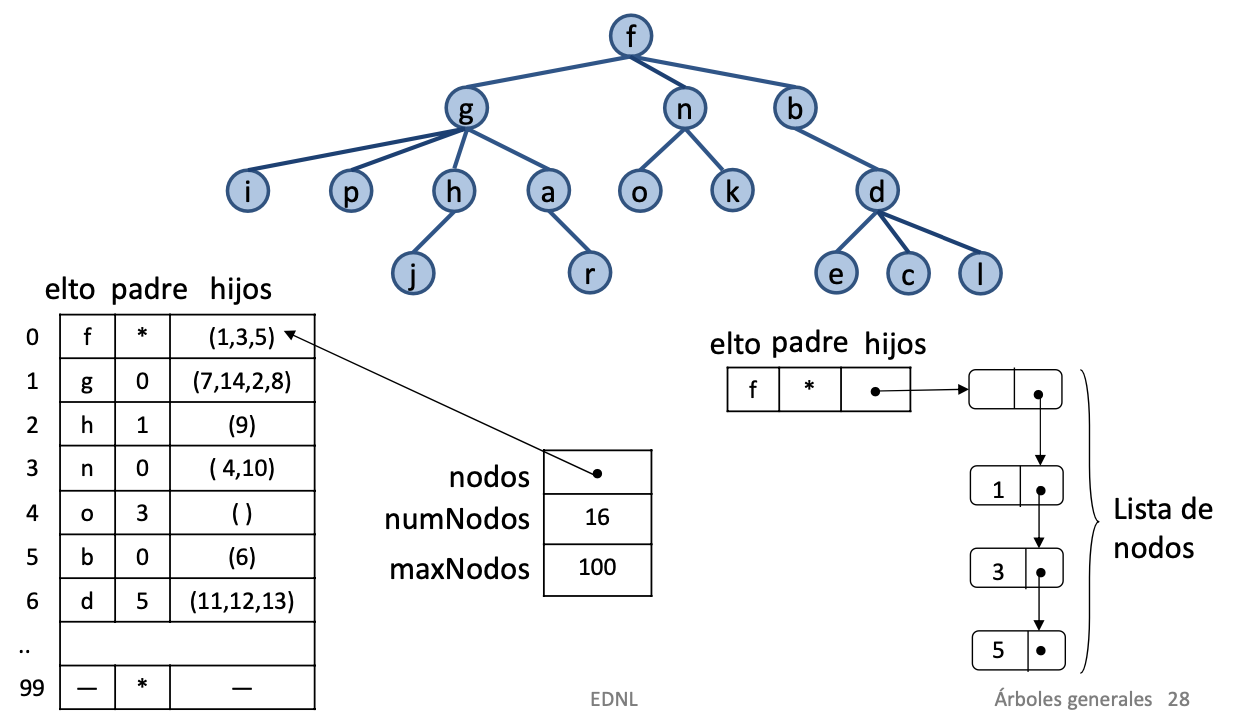
\includegraphics[width=0.75\textwidth]{assets/AgenVec1.png}
  \end{center}
  \caption{Representación de la implementación vectorial mediante lista de hijos.}
\end{figure}

En la parte privada de la implementación de dicho TAD vamos a encontrar el elementos que se almacena, el nodo padre y la lista de los diferentes hijos de cada nodo, todo almacenado en celdas:
\begin{minted}[breaklines]{C++}
template <typename T> class Agen{
  public:
    //Métodos vistos en la especificación del TAD
  private:
    struct celda{
      T elto; //elemento
      nodo padre
      Lista<nodo>hijos;
    };
    celda *nodos; //Vector de nodos
    size_t maxNodos; //Tamaño de vector (árbol)
    size_t numNodos; //Número de nodos en el árbol
};
\end{minted}


\subsection{Implementación mediante celdas enlazadas}
Esta implementación es muy parecida a la implementación mediante celdas enlazadas en árboles binarios, la única diferencia es que en la parte privada no almacenamos hijos derechos, si no que almacenamos hermanos derechos, ya que en nuestro TAD, el concepto de hijo derecho ya no tiene sentido.

\begin{figure}[h]
  \begin{center}
    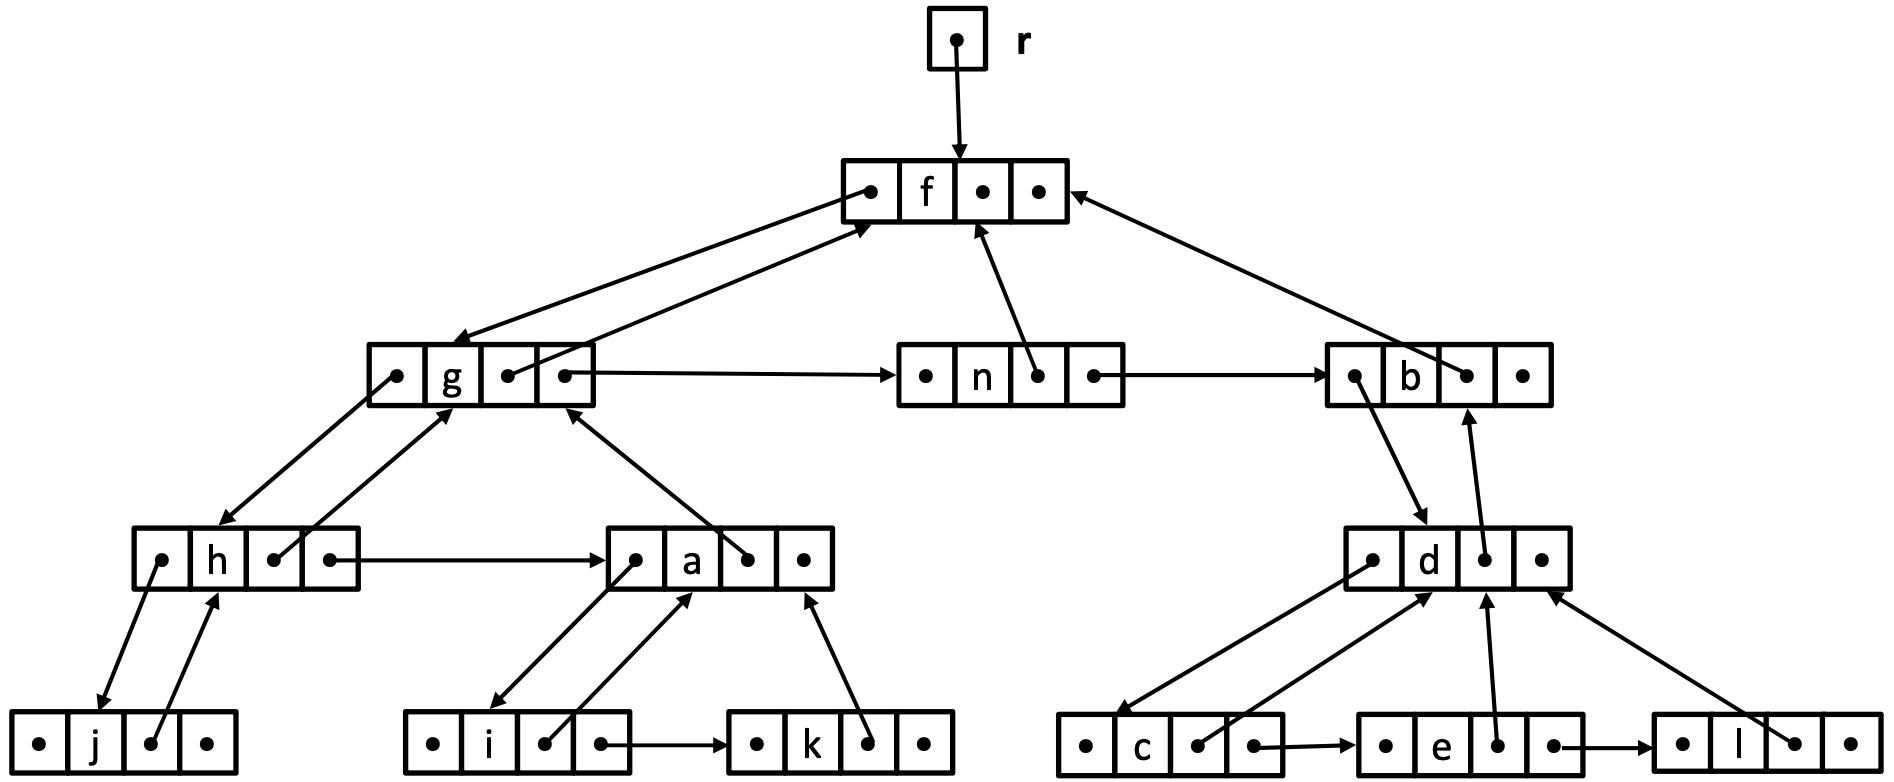
\includegraphics[width=.7\textwidth]{assets/AgenEnla.png}
  \end{center}
  \caption{Representación de la implementación mediante celdas enlazadas}
\end{figure}

Por tanto, la parte privada del TAD nos quedaría:
\begin{verbatim}
template <typename T> class Agen{
  public:
    //Métodos vistos en la especificación del TAD
  private:
    struct celda{
      T elto;
      nodo padre,hizq,heder;
      celda(const T& e, nodo p = NODO_NULO):elto(e),padre(p),
        hizq(NODO_NULO),heder(NODO_NULO){}
    };
    nodo r; //nodo raíz del árbol
};
\end{verbatim}



